\clearpage

\renewcommand{\ChapTitle}{Linear Independence}
\renewcommand{\SectionTitle}{Linear Independence}

\chapter{\ChapTitle}
\section{\SectionTitle}
\horizontalline{0}{0}

\subsection{Assigned Reading}

The reading assignments for this week can be found below:

\begin{itemize}
    \item \textbf{Sections 5.1, 5.2, 5.3, 5.4} from VMLS.
\end{itemize}

\subsection{Piazza}

Must post / respond to at least \textbf{four} Piazza posts this week. \due{(9/29/23)} \cbox{piazza-week5}

\subsection{Lectures}

The lectures for this week and their links can be found below:

\begin{itemize}
    \item \href{https://applied.cs.colorado.edu/mod/hvp/view.php?id=50717}{5.1 - Linear Independence} $\approx$ 13 min.
    \item \href{https://applied.cs.colorado.edu/mod/hvp/view.php?id=50718}{5.2 - Basis} $\approx$ 16 min.
    \item \href{https://applied.cs.colorado.edu/mod/hvp/view.php?id=50719}{5.3 - Orthogonal Vectors} $\approx$ 18 min.
    \item \href{https://applied.cs.colorado.edu/mod/hvp/view.php?id=50720}{5.4 - Gram Schmidt Algorithm} $\approx$ 14 min.
    \item \href{https://applied.cs.colorado.edu/mod/hvp/view.php?id=50721}{5.5 - Complexity} $\approx$ 11 min.
    \item \href{https://applied.cs.colorado.edu/mod/hvp/view.php?id=50722}{Random Exercise Chapter 5} $\approx$ 17 min.
\end{itemize}

\subsection{Assignments}

The assignment for this week is \pdflink{\AssDir Assignment 5 - Linear Independence.pdf}{Assignment 5 - Linear Independence} \due{(10/3/23)} \cbox{assignment-week5}

\subsection{Quiz}

The quiz for this week is \href{https://applied.cs.colorado.edu/mod/quiz/view.php?id=50725}{Chapter 5} \textbullet \pdflink{\QuizDir Quiz 5 - Linear Independence.pdf}{Quiz 5 - Linear Independence} \due{(10/2/23)} \cbox{quiz-week5}

\subsection{Chapter Summary}

The chapter that we will review this week is \textbf{VMLS Chapter 5 - Linear Independence}. The first section that we will cover is \textbf{VMLS Section 5.1 - Linear Independence}.

\begin{notes}{VMLS Section 5.1 - Linear Independence}
    \subsubsection*{Overview}

    Linear independence is a fundamental concept in linear algebra that plays a central role in various mathematical and scientific fields. It provides a powerful framework for understanding the 
    relationships between vectors within a vector space and forms the basis for many key concepts and operations in linear algebra.

    One of the primary implications of linear independence is that it allows us to express vectors in a unique and efficient manner. When a set of vectors is linearly independent, each vector 
    contributes a distinct direction or piece of information to the vector space. This uniqueness is valuable in representing data or systems of equations. For example, in the context of data analysis, 
    linearly independent vectors can help us capture different features or dimensions of a dataset without redundancy. In contrast, linearly dependent vectors can introduce redundancy, making it more 
    challenging to interpret or work with the data effectively.
    
    Moreover, linear independence is closely related to the concept of a basis in linear algebra. A basis is a set of linearly independent vectors that spans a vector space, meaning that any vector 
    in that space can be expressed as a unique linear combination of the basis vectors. Bases are essential because they provide a concise and systematic way to represent vectors within a space. For 
    example, the standard unit vectors in Euclidean space (e.g., (1, 0, 0) and (0, 1, 0) in three-dimensional space) form a basis, allowing us to describe any point in that space using linear 
    combinations of these unit vectors.
    
    Additionally, linear independence is crucial for solving systems of linear equations. When vectors are linearly independent, the system of equations they represent has a unique solution. This 
    property is essential in various scientific and engineering applications, such as solving electrical circuits, analyzing chemical reactions, or optimizing economic models. In contrast, linear 
    dependence in a system of equations can lead to multiple solutions or no solution at all, making it harder to predict or control the behavior of the system.
    
    Linear independence is a foundational concept in linear algebra that underpins many aspects of mathematics and science. It enables us to efficiently represent vectors, construct bases, and solve 
    systems of equations. Whether in data analysis, engineering, physics, or computer science, an understanding of linear independence is essential for making sense of complex mathematical structures 
    and real-world problems.

    \begin{highlight}[Linear Independence Definition]
        For a collection of vectors to be considered \textit{\textbf{linearly independent}} of one another, the collection of vectors must not be linearly dependent. Mathematically this means

        \begin{equation*}
            \sum_{i = 1}^{k} \beta_{i}a_{i} = 0
        \end{equation*}
        where the above equation is only valid if $\beta_{i} = \dots = \beta_{k} = 0$. For a collection of vectors to be \textit{\textbf{linearly dependent}}, the above equation is valid where not all
        of the coefficients $\beta$ are equal to zero. Namely, $\beta_{i} \neq \dots \neq \beta_{k} \neq 0$.
    \end{highlight}
\end{notes}

The next section that we will cover is \textbf{VMLS Section 5.2 - Basis}.

\begin{notes}{VMLS Section 5.2 - Basis}
    \subsubsection*{Overview}

    In the realm of linear algebra, the concept of a basis is fundamental and plays a pivotal role in understanding vector spaces and linear transformations. A basis is essentially a set of vectors 
    that possesses unique and essential properties, making it a cornerstone of vector space theory.

    One of the key characteristics of a basis is linear independence. Linear independence ensures that no vector in the basis can be expressed as a linear combination of the others. In simpler terms, 
    the basis vectors are distinct and do not overlap in their representation of directions within the vector space. This property is crucial because it guarantees that each vector in the space can 
    be uniquely represented using the basis vectors. It's akin to having a set of directions where no two directions are redundant.
    
    Another crucial property of a basis is its spanning ability. A basis should be capable of representing every vector within the vector space by forming linear combinations of its constituent 
    vectors. This means that the basis vectors collectively cover the entire vector space, and any vector within that space can be expressed as a unique combination of these basis vectors. Think of 
    it as having a versatile toolbox of vectors that can be used to build any vector you might encounter in the space.
    
    Bases are not arbitrary sets of vectors; they are meticulously constructed to satisfy these properties while being as minimal as possible. In other words, a basis should have the smallest number 
    of vectors needed to span the entire space while preserving linear independence. This minimalist approach ensures that the basis is efficient and concise in representing the vector space.
    
    Different vector spaces can have different types of bases. For example, in Euclidean space ($R^n$), the standard unit vectors (e.g., [1, 0, 0], [0, 1, 0], [0, 0, 1] for $R^3$) form a natural basis. 
    In the space of polynomials of degree at most n, the monomials $\{1, x, x^{2}, \dots, x^{n}\}$ can serve as a basis. These bases are tailored to the specific characteristics of their respective 
    vector spaces.
    
    In practice, bases are invaluable for solving linear equations, diagonalizing matrices, and understanding linear transformations. They provide structured and systematic ways to work with vectors 
    and linear operators, simplifying complex problems by breaking them down into more manageable components. In essence, bases are the foundation upon which much of linear algebra is built, making 
    them an essential concept for anyone delving into this mathematical field.

    \begin{highlight}[Basis Example]
        In linear algebra, a basis is a fundamental concept that forms the building blocks for vector spaces. A basis is a set of vectors that can be used to represent any vector within that vector space 
        uniquely. To visualize this concept, let's consider a 2D vector space.
    
        \begin{center}
            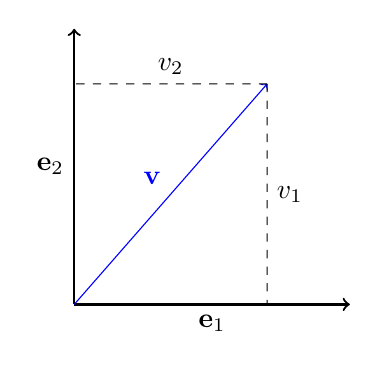
\begin{tikzpicture}[scale=3.5]
                % Define basis vectors
                \coordinate (origin) at (0, 0);
                \coordinate (e1) at (1, 0);
                \coordinate (e2) at (0, 1);
                
                % Draw basis vectors
                \draw[->, thick] (origin) -- (e1) node[midway, below]{$\mathbf{e}_1$};
                \draw[->, thick] (origin) -- (e2) node[midway, left]{$\mathbf{e}_2$};
                
                % Draw vector v in terms of the basis
                \coordinate (v) at (0.7, 0.8);
                \draw[->, blue] (origin) -- (v) node[midway, above left]{$\mathbf{v}$};
                
                % Dashed lines to represent components
                \draw[dashed] (v) -- (0.7, 0) node[midway, right]{$v_1$};
                \draw[dashed] (v) -- (0, 0.8) node[midway, above]{$v_2$};
            \end{tikzpicture}
        \end{center}
    
        In the example provided, we have a 2D basis consisting of two vectors, $\mathbf{e}_1$ and $\mathbf{e}_2$. These basis vectors span the entire 2D space, meaning that any vector in this space can be 
        expressed as a unique combination of these basis vectors. In this case, $\mathbf{e}_1$ points along the x-axis, and $\mathbf{e}_2$ points along the y-axis.

        We also have a vector $\mathbf{v}$, represented in blue, which we want to express in terms of the basis vectors. This involves finding two scalars, $v_1$ and $v_2$, such that $\mathbf{v} = v_1\mathbf{e}_1 
        + v_2\mathbf{e}_2$. The dashed lines in the diagram represent these components: $v_1$ is the length along $\mathbf{e}_1$, and $v_2$ is the length along $\mathbf{e}_2$.

        This illustration demonstrates how vectors within a vector space can be uniquely represented using a basis. The coefficients $v_1$ and $v_2$ are the coordinates of the vector $\mathbf{v}$ with respect 
        to the basis vectors $\mathbf{e}_1$ and $\mathbf{e}_2$, respectively. The concept of a basis is crucial in linear algebra as it forms the foundation for various operations and transformations within 
        vector spaces.
    \end{highlight}

    Consequently, there is a way that we can represent a vector as a linear combination of vectors for a given basis.

    \begin{highlight}[Basis Representation]
        For any $n$-vector $b$, we can write $b$ as 

        \begin{equation*}
            b = b_{1}e_{1} + \dots + b_{n}e_{n}
        \end{equation*}
        where $e_{i}$ are the basis of $b$. In this context $\mathbf{e}$, represents unit vectors in this space.
    \end{highlight}
\end{notes}

The next section that we will cover is \textbf{VMLS Section 5.3 - Orthonormal Vectors}.

\begin{notes}{VMLS Section 5.3 - Orthonormal Vectors}
    \subsubsection*{Overview}

    Orthogonal vectors are a fundamental concept in linear algebra, representing vectors that are mutually perpendicular to each other. In other words, orthogonal vectors have a dot product of zero, 
    which indicates that the angle between them is 90 degrees, forming a right angle. This geometric property makes them particularly useful in various mathematical and engineering applications.

    Orthogonal vectors are essential in defining orthogonal bases for vector spaces. An orthogonal basis is a set of vectors where each vector is orthogonal to all others, and it can simplify vector 
    calculations significantly. In such bases, finding the coefficients to represent a vector becomes straightforward, often involving simple dot products.

    One special case of orthogonal vectors is orthonormal vectors, where orthogonal vectors have unit length, making them particularly convenient for calculations. Orthonormal bases are common in 
    applications like linear transformations and signal processing, where they simplify computations and help maintain vector magnitudes.

    Orthogonal vectors are vectors that are perpendicular to each other, with a dot product of zero. They play a crucial role in linear algebra, forming the basis for orthonormal bases that simplify 
    vector computations and have applications in various fields, including physics, engineering, and computer science.

    \subsubsection*{Orthonormal Basis}

    An orthonormal basis is a special type of basis in linear algebra that combines two essential properties: orthogonality and normalization. In an orthonormal basis, the basis vectors are not only 
    mutually orthogonal (perpendicular to each other) but also normalized (each vector has a magnitude of 1). These two properties make orthonormal bases particularly useful in various mathematical 
    and engineering applications.

    The orthogonality property means that the dot product of any two distinct basis vectors is zero, indicating that they are geometrically perpendicular to each other. This property simplifies vector 
    calculations significantly, making it easier to find coefficients when representing a vector in this basis. Additionally, the normalization property ensures that the basis vectors have unit length, 
    which simplifies magnitude and projection calculations.
    
    Orthonormal bases are especially valuable in linear transformations, where they simplify the transformation process and help maintain the magnitudes of vectors. They are commonly used in signal 
    processing, quantum mechanics, and numerical methods. In quantum mechanics, for example, the states of a quantum system are often represented using an orthonormal basis, simplifying calculations 
    related to measurements and state transformations.
    
    An orthonormal basis consists of vectors that are both orthogonal and normalized. These bases are instrumental in linear algebra and various scientific and engineering disciplines, as they simplify 
    calculations, facilitate vector representations, and ensure consistent magnitudes in mathematical operations.

    \begin{highlight}[Orthonormal Basis]
        To represent an $n$-vector $x$ with an orthonormal basis $a_{1}, \dots, a_{n}$ we use

        \begin{equation*}
            x = \sum_{i = 1}^{n} (a_{i}^{T}x)a_{i}.
        \end{equation*}
        $x$ is expressed as a linear combination of $a_{1}, \dots, a_{n}$.
    \end{highlight}
\end{notes}

The last section that we will cover is \textbf{VMLS Section 5.4 - Gram-Schmidt Algorithm}

\begin{notes}{VMLS Section 5.4 - Gram-Schmidt Algorithm}
    \subsubsection*{Overview}

    The Gram-Schmidt algorithm is a fundamental technique in linear algebra used to transform a set of linearly independent vectors into an orthonormal basis. This process is crucial in various applications, 
    including solving systems of linear equations, eigenvalue problems, and signal processing. The algorithm works by taking a set of linearly independent vectors and systematically orthogonalizing and 
    normalizing them to create a new set of vectors that are both orthogonal (perpendicular) and normalized (unit length).

    The Gram-Schmidt process begins with the first vector in the original set, which is automatically included in the new orthonormal basis as the first vector. Subsequent vectors are processed one by one. 
    For each vector, the algorithm subtracts its projections onto the previously processed vectors from itself, effectively making it orthogonal to those vectors. Then, it normalizes the resulting orthogonal 
    vector to ensure unit length.
    
    Mathematically, the Gram-Schmidt algorithm takes a set of vectors $\{v_{1}, \dots , v_{k}\}$ and transforms them into an orthonormal basis $\{u_{1}, \dots, u_{k}\}$. The resulting basis vectors satisfy 
    two crucial properties: they are mutually orthogonal, meaning their dot products are zero for different vectors, and they are normalized, having a magnitude of 1.
    
    The Gram-Schmidt algorithm is a valuable tool for a wide range of applications in linear algebra and beyond. It helps simplify calculations, particularly in solving linear systems and finding eigenvalues 
    and eigenvectors. Additionally, it plays a vital role in signal processing, quantum mechanics, and various scientific and engineering fields where orthogonal and normalized bases are essential.
    
    The Gram-Schmidt algorithm is a method for converting a set of linearly independent vectors into an orthonormal basis. By ensuring orthogonality and normalization, it simplifies mathematical operations 
    and is a fundamental tool in linear algebra and various scientific disciplines.

    \begin{highlight}[Gram-Schmidt Algorithm]
        Given n-vectors $\mathbf{a}_1, \ldots, \mathbf{a}_k$ for $i = 1, \ldots, k$, perform the following steps:

        \begin{enumerate}
            \item \textbf{Orthogonalization:} $\mathbf{q}_i = \mathbf{a}_i - (\mathbf{q}_1^T \mathbf{a}_i)\mathbf{q}_1 - \ldots - (\mathbf{q}_{i-1}^T \mathbf{a}_i)\mathbf{q}_{i-1}$
            \item \textbf{Linear Independence:} If $\mathbf{q}_i = \mathbf{0}$, quit.
            \item \textbf{Normalization:} $\mathbf{q}_i = \frac{\mathbf{\tilde{q}}_i}{\|\mathbf{\tilde{q}}_i\|}$
        \end{enumerate}

    \end{highlight}
\end{notes}